\documentclass[11pt]{article}

\usepackage[margin=1in]{geometry}
\usepackage{graphicx}
\usepackage{booktabs}
\usepackage{amsmath}
\usepackage{amssymb}
\usepackage{caption}
\usepackage[hidelinks]{hyperref}
\usepackage{times}
\usepackage{longtable}

\setlength{\parindent}{0pt}
\setlength{\parskip}{0.72em}
\captionsetup{font=small,labelfont=bf,skip=4pt}
\renewcommand{\arraystretch}{1.08}
\renewcommand{\topfraction}{0.92}
\renewcommand{\bottomfraction}{0.85}
\renewcommand{\textfraction}{0.06}
\renewcommand{\floatpagefraction}{0.80}

\title{\vspace{-2em}When the Budget Is Actually Spent:\\
Forced Reasoning Depth against Agents, Rounds, and Sampling}
\author{Study \texttt{openrouter\_forced\_budget\_v2}}
\date{18 September 2026}

\begin{document}
\maketitle
\vspace{-1.5em}

\section*{Abstract}

A fixed inference budget can buy more agents, more rounds of revision, more independent samples read
out by a vote, or a longer chain of reasoning inside a single call. The first study in this series
(v1, \texttt{openrouter\_agent\_\allowbreak allocation\_v1}) compared these at a nominal budget
$C = B \cdot R \cdot A$ and concluded that the binding constraint was \emph{selection}: sampling generated
the right answer far more often than any readout delivered it, and no allocation of compute changed that.
Its reasoning allowance $A$, however, was a cap the model was free to leave unspent, and it did: a call
allowed 16,384 reasoning tokens spent 2,774.

This study forces every generation to spend exactly its budget (a logit bias bans the end of reasoning until
the budget is exhausted; the model sees one prompt and no injected text), which makes the budget $C$ real
for every configuration, deep calls included. All 13,344 main-run generations realized
exactly their budget. It reruns the full v1 grid of 96 configurations with
Qwen3.8-27B on 96 items from four hard benchmarks (AIME 2025 and 2026, HMMT February 2025 and
2026, Omni-MATH at difficulty 7 and above, GPQA-Diamond) at $A = 1024$ tokens per call, for
\$70.00.

We ask three questions. \emph{How does pass@$k$ at budget $A$ compare with every other way of spending the
same compute?} On the four-benchmark macro, at every budget that includes a deep call ($2A$ to $25A$), exactly
one configuration delivers more than pass@$k$ of independent 1024-token samples: the single deep call. At $16A$ pass@16 is
0.580 while a vote over the same sixteen samples delivers
0.417, the best revision chain 0.525, the best
team 0.479, and one 16,384-token call 0.792.

\emph{Can a structured allocation close the generation-selection gap?} We decompose every configuration
into what it generates (the coverage of all candidates it produced) and what it delivers. Structured
revision generates more than sampling (a revision chain's candidates cover the answer
6.0 points more often than pass@$k$ on average)
but loses most of it at selection. Selection cannot close the gap from the width side: even a perfect
verifier over sixteen samples delivers 0.562, and over every candidate a
sixteen-call revision chain produced 0.646, both below the deep call.
The gap closes, and is overshot, only by moving compute into depth, where generation and selection
coincide: a single call has nothing to select among. 37 of the 96 items have
no correct answer among all 25 samples; the deep call at $16A$ solves 23 of
them.

\emph{What trends emerge?} Deep calls gain 11.0 accuracy points per
doubling of compute, against 5.7 for the pass@$k$ ceiling of
sampling, 4.8 for revision and
2.0 for the vote. The advantage is carried by competition
mathematics; on GPQA-Diamond, where short samples already reach the answer, the problem remains one of
selection, as in v1. Revision's gains come in its first few steps; peer exposure now helps slightly;
combining deep calls of different depths adds almost nothing, because they succeed and fail on the same
items; and long forced calls that fall into repetition are the ones that had already solved the problem.

\section{Methods}

\subsection{Why a second study}

In v1 the per-call reasoning allowance was a soft request to Gemini 2.5 Flash-Lite. Realized reasoning
flattened at a few thousand tokens however much was requested (Figure~\ref{fig:v1v2}a), so the
\texttt{deep}/$m$ family spent a fraction of its nominal budget and every iso-compute comparison involving
it compared unequal amounts of computation. v1's finding that ``one deep call matches the best
orchestration'' was therefore a statement about a call that was not deep. This study keeps v1's design,
protocols, prompts, selectors and estimators, and changes three things: the budget is enforced, the
model is an open-weight reasoning model whose decoding can be controlled, and the benchmarks are hard
enough that a forced budget cuts reasoning short rather than padding a finished answer.

\begin{figure}[htbp]
\centering
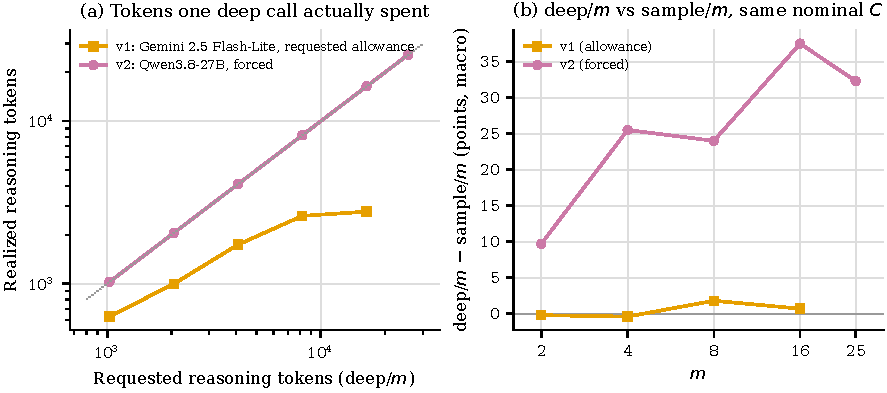
\includegraphics[width=\textwidth]{figures/f4_requested_vs_realized.pdf}
\caption{(a) Reasoning tokens one deep call actually spent against the tokens requested: v1 on its main
panel (Gemini 2.5 Flash-Lite, a soft allowance) and v2 (Qwen3.8-27B, forced). The dotted line is equality.
(b) The consequence for the headline comparison: deep/$m$ minus sample/$m$ on each study's macro. The
two studies differ in model and benchmarks, so (b) contrasts what each design could measure, not the same
quantity twice.}
\label{fig:v1v2}
\end{figure}

\subsection{Forcing the budget}

Each generation node is two calls to OpenRouter's \texttt{/completions} endpoint. The THINK call sends
the model's own chat template, rendered from the node's system and user messages and ending with an
opened reasoning block, with a logit bias of $-100$ on the end-of-reasoning token and the two
end-of-sequence tokens, and \texttt{max\_tokens} equal to the node's budget. The model therefore cannot
close its reasoning and the call ends exactly at the budget. The ANSWER call re-sends the same prompt,
the model's reasoning verbatim and the closing tag, and lets the model write its visible answer freely
under a 4096-token cap. The model is never shown a new instruction or any injected text; the only seam is
that the reasoning is re-tokenized, which adds two or three prompt tokens.

Many OpenRouter endpoints list \texttt{logit\_bias} as supported but silently ignore it, which a +100
bias on an ordinary word exposes at once. Every endpoint was screened this way before use, and each
dispatcher re-ran the screen (together with an exact-length forced call and an answer check) before any
paid work; the screen refused to dispatch into one transient provider outage during the pilot. A THINK
call that ends short of its budget, which happens when a provider cuts a stream, is treated as a
transport failure and retried, never counted. The 131 retried attempts in the main run
cost \$1.02.

The result is exact: every one of the 13,344 main-run generations realized exactly its
reasoning budget (0 exceptions). The budget $C = B\cdot R\cdot A$
of every configuration below is therefore both requested and realized.

\subsection{Model, benchmarks and panels}

Generations come from \texttt{qwen/qwen3.8-27b} at the model's recommended sampling (temperature 1.0,
nucleus 0.95, top-$k$ 20), with the provider pinned per item, fallbacks disabled and response caching
off. Two providers served the run concurrently, each on its own disjoint set of items: Mancer
(58 main items) and Parasail (38). Because every item stays on
one provider, every within-item contrast is same-provider.

Four benchmarks are scored, 24 main items each: AIME 2025 and 2026 and HMMT
February 2025 and 2026 (graded by Math-Verify), Omni-MATH problems of difficulty 7 or more (Math-Verify,
with items whose gold answer is prose or unparseable excluded before any generation), and GPQA-Diamond
(four options shuffled once per item with a fixed seed, exact option match). The panel was drawn by the
harness's frozen, stratified procedure; no item was chosen by model performance.

A pre-registered calibration on eight development items per benchmark (disjoint from the main panel)
required forced pass@1 at $A=1024$ between 0.15 and 0.85 for each benchmark to stay; all four passed
(Table~\ref{tab:cal}). The same calibration ran one unforced generation per item, which shows the regime:
left to itself the model reasons for thousands to tens of thousands of tokens on these problems, so a
forced $A = 1024$ truncates each call hard, and the deep calls up to $25A$ mostly stay at or below the
length the model would choose.

\begin{table}[htbp]
\centering
\small
\begin{tabular}{lrrrr}
\toprule
Benchmark & forced pass@1 ($A$=1024) & natural pass@1 & natural reasoning, median & mean \\
\midrule
AIME 25+26 & 0.312 & 0.875 & 5,550 & 10,844 \\
HMMT Feb 25+26 & 0.250 & 0.625 & 8,858 & 14,389 \\
Omni-MATH $\geq$7 & 0.188 & 0.250 & 29,696 & 25,475 \\
GPQA-Diamond & 0.500 & 0.625 & 14,069 & 16,231 \\
\bottomrule
\end{tabular}
\caption{Calibration on 8 development items per benchmark (not the main panel). Natural generations were
capped at 25,600 reasoning plus 4,096 answer tokens; on Omni-MATH the median call reached that cap, so its
natural length is a lower bound.}
\label{tab:cal}
\end{table}

\subsection{The compute accounting}

Each configuration is a triple $(B, R, A)$ and its budget is their product, read from the sealed
tables rather than parsed from names:

\begin{center}
\small
\begin{tabular}{llccc}
\toprule
Family & Notation & $B$ & $R$ & $C$ \\
\midrule
Independent samples, plurality vote & \texttt{sample/k} & $k$ & 1 & $kA$ \\
One agent revising its own answer & \texttt{private\_single/t} & 1 & $t$ & $tA$ \\
Team, no peer exposure & \texttt{private\_team/n/r} & $n$ & $1+r$ & $n(1+r)A$ \\
Team, peer exposure & \texttt{peer/n/r} & $n$ & $1+r$ & $n(1+r)A$ \\
One deeper call & \texttt{deep/m} & 1 & 1 & $mA$ \\
\bottomrule
\end{tabular}
\end{center}

$A = 1024$ throughout, $m \in \{1,2,4,8,16,25\}$ (deep/25 is new, so that depth reaches the 25-generation
budgets), teams have $n \in \{2,\dots,5\}$ and $r \in \{1,\dots,4\}$, and deep/1 is root[0] of the
sampling bank. Figure~\ref{fig:design} shows the design: five budget levels ($C/A \in \{2,4,8,16,25\}$)
carry a deep call alongside several multi-call allocations, which is where depth and width meet at equal
realized compute.

\begin{figure}[htbp]
\centering
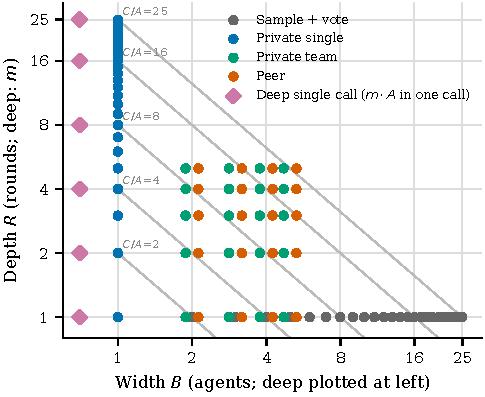
\includegraphics[width=0.55\textwidth]{figures/f1_design.pdf}
\caption{Every evaluated configuration in the width-depth plane; grey lines are iso-compute contours.
Deep calls are drawn at the left, at height $m$: one call carrying $m$ units of reasoning.}
\label{fig:design}
\end{figure}

\subsection{Generation, selection and the gap}
\label{sec:defs}

Every configuration produces a pool of candidate answers and a selector delivers one of them. We separate
the two:

\begin{itemize}
\item \textbf{Delivered accuracy} is the share of items on which the delivered answer is correct.
\item \textbf{Coverage} is the share of items on which the pool contains at least one correct answer. It
is computed for two pools. The \emph{current} pool is what the configuration's selector actually chooses
from (the last round of a team; the last answer of a revision chain; all $k$ samples of \texttt{sample/k}).
The \emph{archive} pool is every candidate the configuration ever generated (every round of a team, every
step of a chain). Archive coverage measures what the configuration \emph{generated}; delivered accuracy
measures what it \emph{selected}.
\item \textbf{The selection gap} is coverage minus delivered accuracy.
\item \textbf{pass@$k$ at $A$} is the combinatorial estimator $1-\binom{25-c}{k}/\binom{25}{k}$ over the
25-sample bank of independent 1024-token calls, $c$ the number of correct samples. It is the generation
ceiling of spending $C = kA$ on independent samples: the delivered accuracy of a perfect selector.
\item \textbf{Capture} $\eta = (\text{delivered} - \text{pass@1}) / (\text{coverage} - \text{pass@1})$ is
the share of the configuration's own generated headroom that its selector collects.
\end{itemize}

For a single deep call the pool has one candidate, so coverage equals delivered accuracy and the selection
gap is zero by construction: a deep call trades width for depth and has nothing to select among.

To ask what better selection could recover without new generation, we model a verifier that scores each
candidate and picks the highest: correct and wrong candidates have normally distributed scores separated so
that a random correct candidate outscores a random wrong one with probability AUC. AUC 0.5 is a random pick
from the pool; AUC 1 is an oracle that delivers exactly the coverage. For a pool of $n$ candidates with $c$
correct, the probability of delivering a correct answer is computed by simulation and averaged over items.

\subsection{Estimation and multiplicity}

A configuration delivers one answer per item: plurality vote for sampling and team arms, the last
answer for private chains and deep calls. Invalid or unparseable outputs count as incorrect. All
intervals are percentile intervals from a 10,000-replicate item-clustered bootstrap, stratified by
benchmark; every configuration shares the same resample indices, so differences between configurations
are paired item by item. Macro averages weight the four benchmarks equally.

Two contrasts were frozen before collection (peer against private team at $n=4, r=4$, and the
communicate-then-private decomposition); they are quoted from the sealed contrast table. Everything else
is exploratory. In the amplification analysis every configuration is compared with independent sampling
at the same budget, and Benjamini-Hochberg control is applied within each benchmark panel.

\subsection{Limitations}

With 24 items per benchmark one item is 4.2 accuracy points, so single-benchmark differences below
roughly 15 points are not separable from noise; the macro, on 96 items, is the primary lens. Results are
from one mid-sized model and should not be assumed to transfer to larger ones. Forcing the budget is a
decode-time intervention: a forced call is not the call the model would make, and past its natural
length the model can fill the budget with repetition (Section~\ref{sec:loops}). The Math-Verify grader
timed out on 82 of 13,344 generations (0.6\%),
concentrated on two items with extremely long answers; the pre-registered 5-second grading limit was kept
rather than changed after the fact, so 46 of 9,216
configuration outcomes are unknown and are excluded pairwise from intervals (and reported as bounds in
the sealed contrasts). 304 generations (2.3\%) produced no
parseable final answer and score as wrong. This is a token- and dollar-accounted study, not a FLOP-matched
one.

\section{Results}

The results are organised around the three questions. Section~\ref{sec:dom} shows the headline. Sections
\ref{sec:passk} to \ref{sec:vote} compare pass@$k$ at $A$ with every allocation of the same compute and
decompose each allocation into generation and selection: whether better selection could close the gap
(\ref{sec:ver}), on which items the gap lives (\ref{sec:strata}) and what a vote knows
(\ref{sec:vote}). Sections \ref{sec:ceiling} and \ref{sec:portf} show that depth passes the sampling ceiling
and ask whether depth itself can be allocated in structured portfolios. Sections \ref{sec:dvw} to
\ref{sec:shape} give the matched-compute contrasts and the trends in scaling, revision dynamics and team
shape; the remaining sections cover repetition, communication, dollars and robustness.

\subsection{Depth dominates at every matched budget}
\label{sec:dom}

Figure~\ref{fig:ladder} is the headline. On the three mathematics benchmarks the deep curve separates from
every other family by the second budget level and keeps climbing, while sampling, teams and even the
oracle ceiling of the sampling bank rise slowly.

\begin{figure}[htbp]
\centering
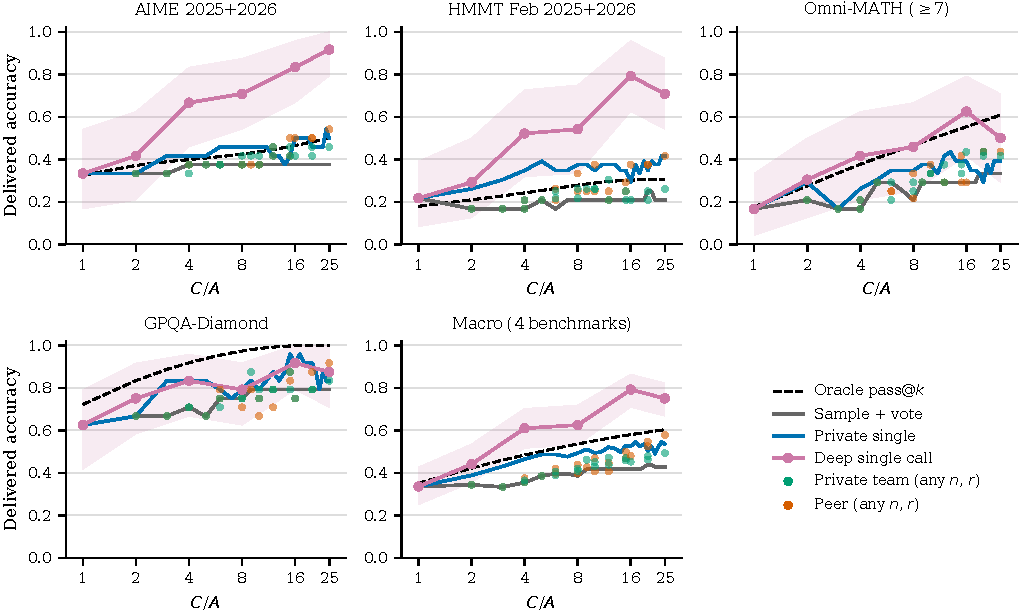
\includegraphics[width=\textwidth]{figures/f2_ladder.pdf}
\caption{Delivered accuracy against realized compute $C/A$. All points at a given $x$ spend the same number
of reasoning tokens. The dashed line is oracle pass@$k$ of the 25-sample bank, an unavailable selector.
The band is the 95\% bootstrap interval of the deep curve; dots are individual team configurations.}
\label{fig:ladder}
\end{figure}

On the macro, one sample delivers 0.336. Sampling with a vote reaches
0.417 at sixteen samples and 0.427 at twenty-five. A single
agent revising its own answer does better, 0.525 after sixteen calls.
The deep call reaches 0.610 at $4A$, 0.625 at $8A$ and
0.792 at $16A$ (95\% CI 0.708 to 0.865),
the best value of any configuration in the design. At $25A$ it delivers 0.750; the
difference from $16A$ is $-$4.2 points (95\% CI
$-$10.4 to +2.1), not
distinguishable from zero.

Per benchmark the pattern is sharp on competition mathematics and absent on GPQA-Diamond
(Table~\ref{tab:headline}). On AIME the deep call climbs to 0.917 at $25A$, while
sampling stays at 0.375 and the sampling oracle reaches only
0.500. On HMMT deep/16 delivers 0.792 against
0.208 for sampling. On Omni-MATH the deep call reaches 0.625
at $16A$ against 0.292. On GPQA-Diamond sampling already starts at
0.625 and its oracle saturates near 1; the best configuration there is
\texttt{private\_single/17} at 0.958, and deep calls and revision chains
are statistically indistinguishable.

\begin{table}[htbp]
\centering
\small
\begin{tabular}{lrrrrrrr}
\toprule
Benchmark & pass@1 & vote@25 & oracle@25 & priv.\ 25 & best team & deep/16 & deep/25 \\
\midrule
AIME 25+26 & 0.333 & 0.375 & 0.500 & 0.500 & 0.542 & 0.833 & 0.917 \\
HMMT Feb 25+26 & 0.217 & 0.208 & 0.304 & 0.417 & 0.417 & 0.792 & 0.708 \\
Omni-MATH $\geq$7 & 0.167 & 0.333 & 0.609 & 0.391 & 0.435 & 0.625 & 0.500 \\
GPQA-Diamond & 0.625 & 0.792 & 1.000 & 0.833 & 0.917 & 0.917 & 0.875 \\
Macro (4) & 0.336 & 0.427 & 0.603 & 0.535 & 0.577 & 0.792 & 0.750 \\
\bottomrule
\end{tabular}

\caption{Delivered accuracy of reference configurations. vote@25 is sample/25; oracle@25 is pass@25 of
the same bank; priv.\ 25 is a 25-call private revision chain; best team is the best peer or private-team
configuration on that row.}
\label{tab:headline}
\end{table}

\subsection{pass@\texorpdfstring{$k$}{k} at \texorpdfstring{$A$}{A} against every allocation of the same compute}
\label{sec:passk}

Table~\ref{tab:rung} places, at each budget $C = kA$ that carries a deep call, the ceiling of independent
sampling (pass@$k$) beside what the vote over those same $k$ samples delivers and what the best revision
chain, the best team and the single deep call deliver with the same total reasoning tokens. The full list
of every configuration at every one of these budgets, with its coverage, is in Appendix~\ref{app:full}.

\begin{table}[htbp]
\centering
\small
\begin{tabular}{rrrrrrrrr}
\toprule
$C/A$ & pass@$k$ & vote@$k$ & \multicolumn{2}{c}{private chain} & \multicolumn{2}{c}{best team} & deep & best non-deep \\
 & & & delivered & coverage & delivered & coverage & & \\ \midrule
2 & 0.422 & 0.344 & 0.388 & 0.430 & 0.344 & 0.440 & 0.441 & 0.388 \\
4 & 0.484 & 0.354 & 0.465 & 0.540 & 0.375 & 0.471 & 0.610 & 0.465 \\
8 & 0.536 & 0.385 & 0.493 & 0.561 & 0.438 & 0.535 & 0.625 & 0.493 \\
16 & 0.580 & 0.417 & 0.525 & 0.657 & 0.479 & 0.615 & 0.792 & 0.525 \\
25 & 0.603 & 0.427 & 0.535 & 0.689 & 0.577 & 0.647 & 0.750 & 0.577 \\
\bottomrule
\end{tabular}

\caption{Macro accuracy at equal realized compute $C = kA$. pass@$k$ is the generation ceiling of $k$
independent 1024-token samples; every other column is delivered accuracy (coverage columns are the share of
items on which the configuration's own candidates, over all its rounds, contained a correct answer).}
\label{tab:rung}
\end{table}

Three facts stand out. First, at every budget only one configuration delivers more than pass@$k$: on the
macro exactly 1 of 7 configurations at
$4A$, 1 of 9 at $8A$,
1 of 6 at $16A$ and
1 of 5 at $25A$, and that one is the
deep call. Pass@$k$ is an upper bound on anything that selects among $k$ independent samples; it is not an
upper bound on anything else, and depth is the only allocation in the design that goes past it.

Second, among the allocations that use several calls, none comes close to the sampling ceiling: at $16A$ the
best of them delivers 0.525 (\texttt{private\_single/16})
against pass@16 of 0.580, and at $25A$ the best,
\texttt{peer/5/4}, delivers 0.577 against
0.603.

Third, several of those allocations \emph{generate} more than pass@$k$ even though they deliver less: at
$16A$ the revision chain's candidates cover 0.657 of items, above
pass@16. The structured allocations do not fail for lack of generation; they fail at turning what they
generate into a delivered answer (Section~\ref{sec:decomp}).

Per benchmark (Table~\ref{tab:rungb}) the pattern holds on AIME and HMMT, where the deep call exceeds pass@$k$
by a wide margin at every budget from $4A$, weakens on Omni-MATH, where pass@25 (0.609)
overtakes the deep call at $25A$ (0.500), and reverses on GPQA-Diamond, where
pass@$k$ is near 1 by $k=8$ and no configuration approaches it.

\begin{table}[htbp]
\centering
\small
\begin{tabular}{llrrrrr}
\toprule
Benchmark & $C/A$ & pass@$k$ & vote@$k$ & private chain & best team & deep \\ \midrule
AIME 25+26 & 4 & 0.399 & 0.375 & 0.417 & 0.375 & 0.667 \\
 & 8 & 0.424 & 0.375 & 0.458 & 0.417 & 0.708 \\
 & 16 & 0.465 & 0.375 & 0.500 & 0.500 & 0.833 \\
 & 25 & 0.500 & 0.375 & 0.500 & 0.542 & 0.917 \\
\addlinespace
HMMT Feb 25+26 & 4 & 0.242 & 0.167 & 0.348 & 0.208 & 0.522 \\
 & 8 & 0.278 & 0.208 & 0.375 & 0.333 & 0.542 \\
 & 16 & 0.302 & 0.208 & 0.292 & 0.375 & 0.792 \\
 & 25 & 0.304 & 0.208 & 0.417 & 0.417 & 0.708 \\
\addlinespace
Omni-MATH $\geq$7 & 4 & 0.376 & 0.167 & 0.261 & 0.208 & 0.417 \\
 & 8 & 0.467 & 0.208 & 0.348 & 0.333 & 0.458 \\
 & 16 & 0.553 & 0.292 & 0.391 & 0.435 & 0.625 \\
 & 25 & 0.609 & 0.333 & 0.391 & 0.435 & 0.500 \\
\addlinespace
GPQA-Diamond & 4 & 0.918 & 0.708 & 0.833 & 0.708 & 0.833 \\
 & 8 & 0.973 & 0.750 & 0.792 & 0.750 & 0.792 \\
 & 16 & 0.998 & 0.792 & 0.917 & 0.750 & 0.917 \\
 & 25 & 1.000 & 0.792 & 0.833 & 0.917 & 0.875 \\
\addlinespace
\bottomrule
\end{tabular}

\caption{Per benchmark, at equal realized compute: pass@$k$ of 1024-token samples against delivered accuracy
of the vote, the private revision chain, the best team and the deep call. 24 items per benchmark.}
\label{tab:rungb}
\end{table}

\subsection{Generation and selection, allocation by allocation}
\label{sec:decomp}

Figure~\ref{fig:plane} places every configuration in the generation-selection plane: archive coverage on the
horizontal axis, delivered accuracy on the vertical. The diagonal is perfect selection. Independent sampling
traces the dashed line from pass@$k$ to vote@$k$; deep calls sit on the diagonal by construction. Every
multi-call configuration lies below the diagonal, and the distance is large.

\begin{figure}[htbp]
\centering
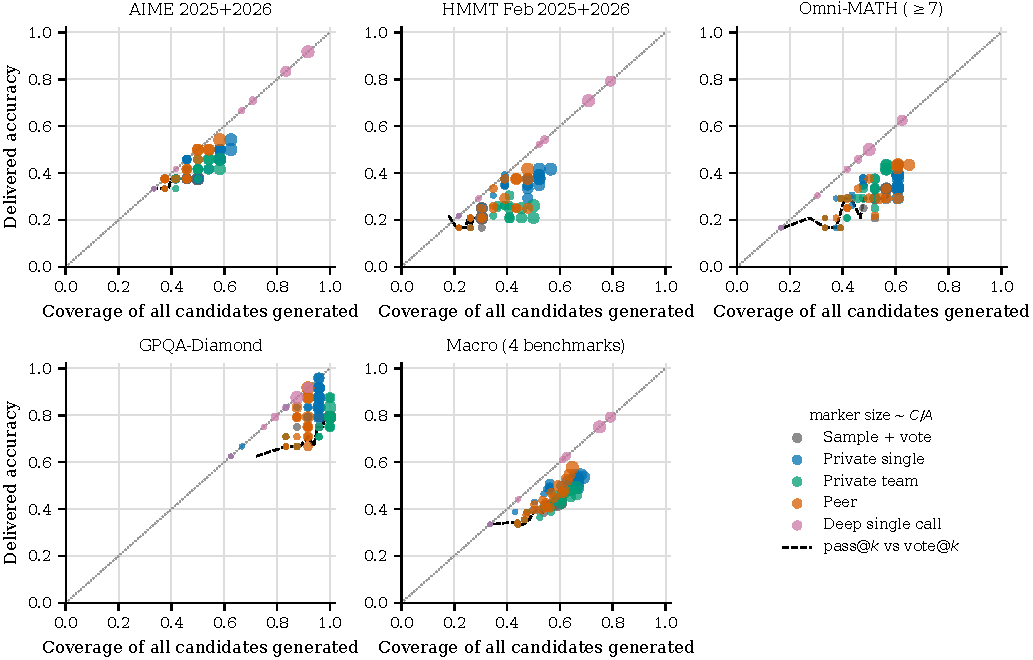
\includegraphics[width=\textwidth]{figures/g1_generation_selection_plane.pdf}
\caption{The generation-selection plane. Each point is one configuration; the horizontal axis is the share of
items on which any candidate it generated (over all rounds) was correct, the vertical axis the share on which
its delivered answer was correct. Points on the dotted diagonal select perfectly. The dashed line connects
pass@$k$ to vote@$k$ for independent sampling.}
\label{fig:plane}
\end{figure}

Averaged over budgets of $4A$ and above on the macro (Figure~\ref{fig:decomp}):

\begin{itemize}
\item \textbf{Independent sampling} generates at the pass@$k$ ceiling by definition and captures
0.342 of its headroom; its selection gap averages
14.6 points.
\item \textbf{The private revision chain} generates \emph{more}: its candidates cover the answer
+6.0 points more often than pass@$k$ at the
same budget, because each step starts from a better draft. It delivers only its last answer, which captures
0.614 of the headroom and leaves a gap of
11.4 points to answers it generated and then revised away.
\item \textbf{Private teams} generate +3.8 points
above pass@$k$ and capture 0.372; the gap averages
15.3 points.
\item \textbf{Peer teams} generate +0.9 points above
pass@$k$ and capture 0.464, better than private teams: seeing each other's
answers makes agents converge, which helps the final vote.
\item \textbf{Communicate-then-private} captures 0.356 and \textbf{pooled
synthesis} 0.441.
\end{itemize}

So the structured allocations of v1's design do move generation above the sampling ceiling, modestly, and
they do not solve selection: every one of them leaves between two fifths and two thirds of its own
generated headroom uncollected.

\begin{figure}[htbp]
\centering
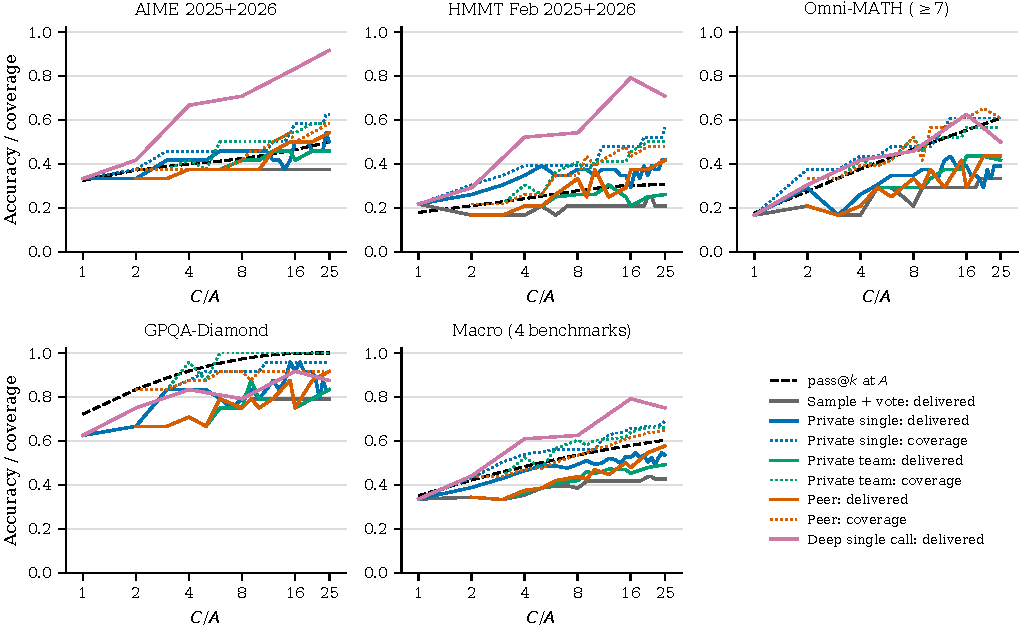
\includegraphics[width=\textwidth]{figures/g2_family_decomposition.pdf}
\caption{Per family, the best delivered accuracy (solid) and the best archive coverage (dotted) at each
budget, against pass@$k$ at $A$ (dashed). The vertical distance between a family's dotted and solid line is
its selection gap.}
\label{fig:decomp}
\end{figure}

\subsection{Could better selection close the gap?}
\label{sec:ver}

If the gap were a selection problem, a better selector over candidates already generated would close it.
Figure~\ref{fig:ver} and Table~\ref{tab:ver} give the macro accuracy that a verifier of a given quality would
deliver from three pools at each budget: the $k$ independent samples, every candidate of a $k$-call revision
chain, and every candidate of the team with the highest coverage at that budget.

\begin{figure}[htbp]
\centering
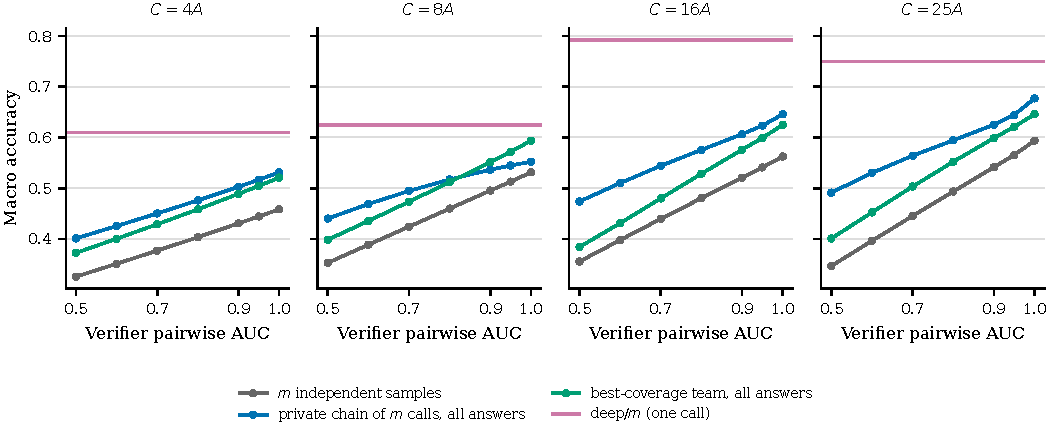
\includegraphics[width=\textwidth]{figures/g3_verifier_sweep.pdf}
\caption{Macro accuracy a verifier of pairwise AUC $a$ would deliver by picking the top-scored candidate from
each pool at equal compute, against the single deep call at the same compute (horizontal line). AUC 1 equals
the pool's coverage.}
\label{fig:ver}
\end{figure}

\begin{table}[htbp]
\centering
\small
\begin{tabular}{llrrrrrrr}
\toprule
$C/A$ & pool & AUC 0.5 & 0.6 & 0.7 & 0.8 & 0.9 & 0.95 & 1.0 \\ \midrule
4 & 4 samples & 0.326 & 0.351 & 0.377 & 0.403 & 0.431 & 0.444 & 0.458 \\
4 & chain of 4, all answers & 0.401 & 0.425 & 0.450 & 0.476 & 0.503 & 0.517 & 0.531 \\
4 & best team, all answers & 0.372 & 0.400 & 0.429 & 0.458 & 0.489 & 0.504 & 0.521 \\
4 & \emph{deep/4, one call} & \multicolumn{7}{c}{0.610} \\
\addlinespace
8 & 8 samples & 0.353 & 0.388 & 0.424 & 0.460 & 0.495 & 0.513 & 0.531 \\
8 & chain of 8, all answers & 0.440 & 0.469 & 0.495 & 0.517 & 0.537 & 0.545 & 0.552 \\
8 & best team, all answers & 0.398 & 0.435 & 0.473 & 0.512 & 0.551 & 0.572 & 0.594 \\
8 & \emph{deep/8, one call} & \multicolumn{7}{c}{0.625} \\
\addlinespace
16 & 16 samples & 0.355 & 0.398 & 0.440 & 0.480 & 0.521 & 0.541 & 0.562 \\
16 & chain of 16, all answers & 0.474 & 0.510 & 0.544 & 0.576 & 0.607 & 0.623 & 0.646 \\
16 & best team, all answers & 0.384 & 0.431 & 0.480 & 0.529 & 0.576 & 0.599 & 0.625 \\
16 & \emph{deep/16, one call} & \multicolumn{7}{c}{0.792} \\
\addlinespace
25 & 25 samples & 0.347 & 0.396 & 0.445 & 0.493 & 0.541 & 0.565 & 0.594 \\
25 & chain of 25, all answers & 0.491 & 0.530 & 0.564 & 0.594 & 0.625 & 0.644 & 0.677 \\
25 & best team, all answers & 0.401 & 0.452 & 0.503 & 0.552 & 0.599 & 0.621 & 0.646 \\
25 & \emph{deep/25, one call} & \multicolumn{7}{c}{0.750} \\
\addlinespace
\bottomrule
\end{tabular}

\caption{Verifier sweep, macro. Rows are pools of candidates already generated; columns are verifier pairwise
AUC. The deep call's accuracy is given for comparison at each budget.}
\label{tab:ver}
\end{table}

No verifier over any of these pools reaches the deep call on the macro at any budget from $4A$. At $16A$ a
realistic verifier (AUC 0.7) over sixteen samples delivers 0.440, a strong one
(AUC 0.9) 0.521, and a perfect one 0.562, against
0.792 for one deep call. The revision chain's archive is the best pool to select from,
but a perfect verifier over it still delivers only 0.646, and over the
best team's candidates 0.625. Perfect selection over sixteen samples falls
23.0 points short of the deep call on the macro. On AIME and HMMT the shortfall is
37.5 and 50.0 points. Only on
GPQA-Diamond does perfect selection over samples beat depth, by +8.3
points at $16A$.

In this regime, then, the gap between what short samples generate and what depth delivers is not a selection
gap at all. It is a generation gap that pass@$k$ hides, because pass@$k$ is the ceiling of one particular
allocation, not of the budget.

\subsection{Where the gap lives: items by difficulty}
\label{sec:strata}

Grouping items by how many of their 25 independent samples were correct shows which items each allocation
wins (Figure~\ref{fig:strata}, Table~\ref{tab:strata}). 37 of the 96 main items
(12 AIME, 16 HMMT,
9 Omni-MATH, 0 GPQA) have
no correct sample at all: no selector over 25 samples, and no amount of voting or verification, can deliver
them. The deep call solves 11 of them at $4A$, 16
at $8A$ and 23 at $16A$; some deep call solves 27.
The 25-call revision chain solves 7.

\begin{figure}[htbp]
\centering
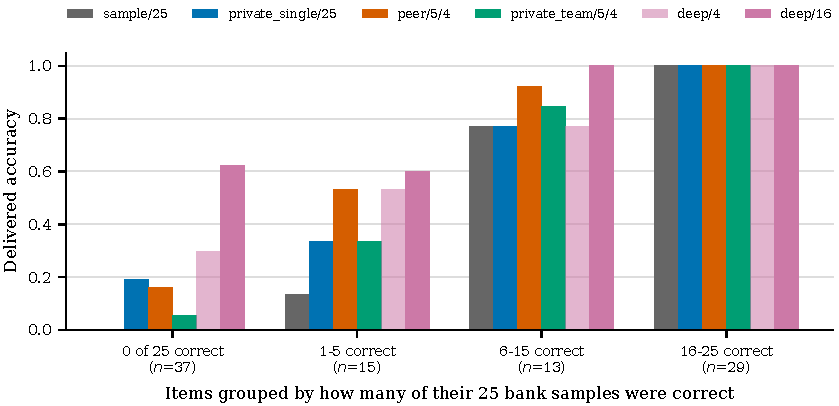
\includegraphics[width=\textwidth]{figures/g4_difficulty_strata.pdf}
\caption{Delivered accuracy by item difficulty, measured as the number of the item's 25 independent
1024-token samples that were correct.}
\label{fig:strata}
\end{figure}

\begin{table}[htbp]
\centering
\small
\begin{tabular}{lrrrrrrrrr}
\toprule
Samples correct & items & vote 25 & chain 25 & peer 5/4 & team 5/4 & deep/4 & deep/8 & deep/16 & deep/25 \\ \midrule
0 of 25 & 37 & 0.000 & 0.189 & 0.162 & 0.054 & 0.297 & 0.432 & 0.622 & 0.568 \\
1-5 & 15 & 0.133 & 0.333 & 0.533 & 0.333 & 0.533 & 0.600 & 0.600 & 0.667 \\
6-15 & 13 & 0.769 & 0.769 & 0.923 & 0.846 & 0.769 & 0.692 & 1.000 & 0.846 \\
16-25 & 29 & 1.000 & 1.000 & 1.000 & 1.000 & 1.000 & 0.897 & 1.000 & 0.966 \\
\bottomrule
\end{tabular}

\caption{Delivered accuracy by item difficulty (number of correct samples among 25).}
\label{tab:strata}
\end{table}

On items that short samples usually solve (16 or more of 25 correct), every allocation is near perfect. On the
middle strata the allocations separate by how well they select. On the items short samples never solve, the
multi-call allocations recover a few, because revising a draft or reading a peer's answer occasionally
produces an answer no independent sample did (the 25-call chain 0.189, the
five-agent peer team 0.162); the deep call recovers most
(0.622 at $16A$). Item by item at $16A$
(94 items with complete data), the deep call and the first sixteen samples both reach the
answer on 49, only the deep call on 25, only the samples on
5, and neither on 15.

\subsection{What a vote knows}
\label{sec:vote}

Plurality voting is a selector with a built-in confidence signal: the share of samples that agree. Among the
25 samples, the plurality answer is almost always right when it holds a large share and almost always wrong
when it holds a small one (Figure~\ref{fig:vote}a). The low-agreement items are exactly the hard ones, and on
those the deep call is still right most of the time: the vote's confidence tells you \emph{when} sampling has
failed, not how to recover. Answer diversity tells the same story (Figure~\ref{fig:vote}b): on items where
the 25 samples produce eight or more distinct answers (the median item has
13 distinct answers among its 25 samples), the samples' coverage and vote collapse
while the deep call does not. Low agreement among short samples is therefore a usable signal for
\emph{routing} an item to depth.

\begin{figure}[htbp]
\centering
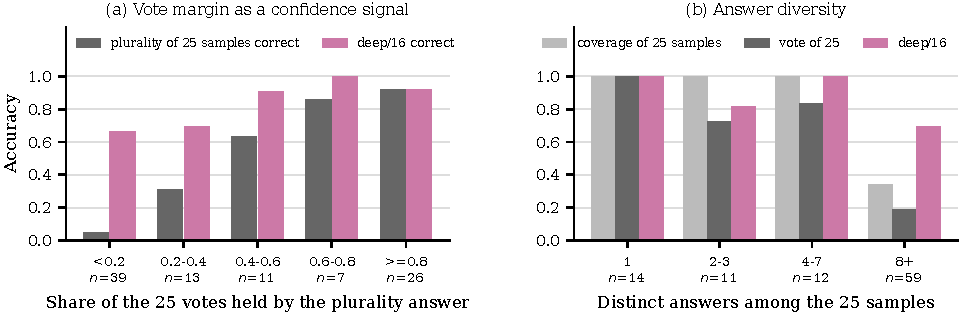
\includegraphics[width=\textwidth]{figures/g5_vote_calibration.pdf}
\caption{(a) Accuracy of the plurality of 25 samples, and of deep/16, by the share of votes the plurality
answer holds. (b) Coverage and vote of 25 samples and accuracy of deep/16, by the number of distinct answers
among the 25 samples. Answer classes group all graded-correct answers together and wrong answers by exact
normalized form.}
\label{fig:vote}
\end{figure}

\subsection{Depth goes past the ceiling of short samples}
\label{sec:ceiling}

In v1 the binding constraint was selection: the sampling bank contained the right answer far more often
than any vote found it. The same gap exists here, and grows with $k$: at $k=25$ oracle pass@$k$ exceeds the
vote readout by 17.6 macro points (Figure~\ref{fig:sel}). But the deep call
does not merely close that gap; it goes past the ceiling. deep/$m$ exceeds oracle pass@$m$ of the sampling
bank by 12.6 points at $m=4$ and 21.2 at $m=16$ on the
macro, and by 49.0 points on HMMT at $m=16$. Twenty-five independent 1024-token
attempts at an HMMT problem contain a correct answer on 0.304 of items; one 16,384-token
attempt is correct on 0.792. The limit of a short sample is not that the right answer is
hard to pick out; it is that a short sample usually does not produce it at all.

\begin{figure}[htbp]
\centering
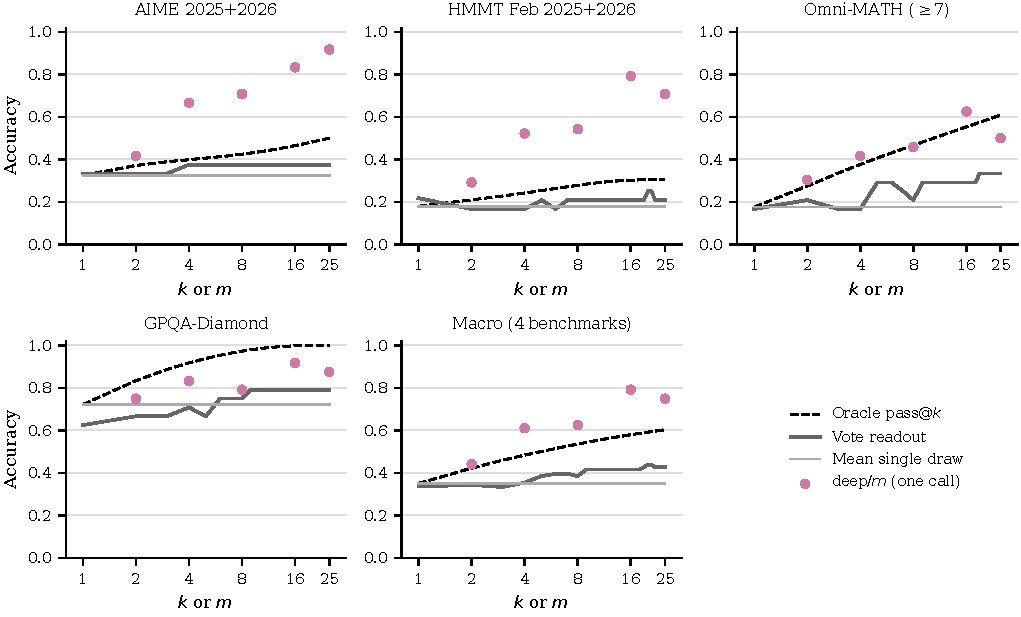
\includegraphics[width=\textwidth]{figures/f6_selection.pdf}
\caption{The sampling bank at $A=1024$: oracle pass@$k$, the vote readout and the mean single draw, with
the deep call at $m$ times the budget overlaid. Points above the dashed line are beyond anything a
selector over $k$ short samples could deliver.}
\label{fig:sel}
\end{figure}

The exception is GPQA-Diamond, where the sampling oracle reaches 1.000 and the deep
call stays below it ($-$8.1 points at $m=16$). A multiple-choice question
whose answer a short sample often reaches is a selection problem, as in v1; a competition problem whose
answer a short sample rarely reaches is a depth problem.

\subsection{Structured allocations of depth}
\label{sec:portf}

If a single deep call wins, the natural next question is whether depth itself can be allocated in structured
ways: several deep calls of different lengths, read out by a vote or by trusting the deepest. The run
collected one deep call per item at each of $2A, 4A, 8A, 16A$ and $25A$ (plus root[0] at $A$), which allows
portfolios of distinct depths to be evaluated without new generation (Figure~\ref{fig:portf},
Table~\ref{tab:portf}).

\begin{figure}[htbp]
\centering
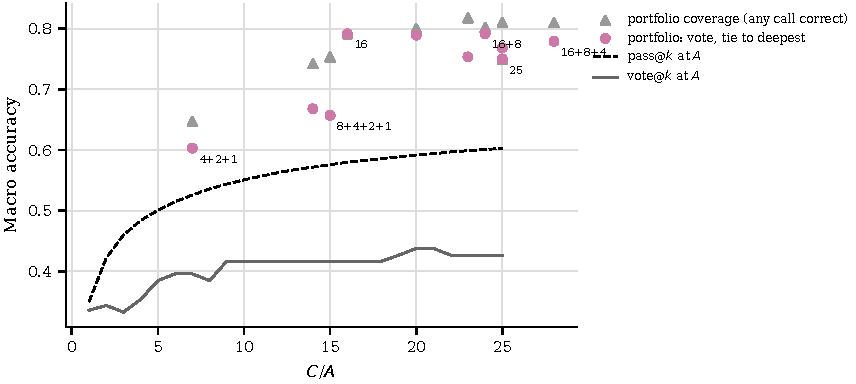
\includegraphics[width=0.72\textwidth]{figures/g6_deep_portfolios.pdf}
\caption{Portfolios of deep calls of different depths (labels: multiples of $A$), against pass@$k$ and
vote@$k$ of 1024-token samples at the same total compute. Triangles: coverage (some call in the portfolio is
correct); circles: plurality vote over the portfolio, ties broken toward the deepest call.}
\label{fig:portf}
\end{figure}

\begin{table}[htbp]
\centering
\small
\begin{tabular}{lrrrrrr}
\toprule
Deep calls (multiples of $A$) & $C/A$ & coverage & deepest & vote & pass@$C$ & vote@$C$ \\ \midrule
4+2+1 & 7 & 0.647 & 0.614 & 0.603 & 0.526 & 0.396 \\
8+4+2 & 14 & 0.742 & 0.636 & 0.668 & 0.572 & 0.417 \\
8+4+2+1 & 15 & 0.753 & 0.636 & 0.657 & 0.576 & 0.417 \\
16 & 16 & 0.792 & 0.792 & 0.792 & 0.580 & 0.417 \\
16+4 & 20 & 0.800 & 0.789 & 0.789 & 0.592 & 0.438 \\
16+4+2+1 & 23 & 0.817 & 0.785 & 0.754 & 0.599 & 0.427 \\
16+8 & 24 & 0.802 & 0.792 & 0.792 & 0.601 & 0.427 \\
16+8+1 & 25 & 0.810 & 0.789 & 0.769 & 0.603 & 0.427 \\
25 & 25 & 0.750 & 0.750 & 0.750 & 0.603 & 0.427 \\
16+8+4 & 28 & 0.810 & 0.789 & 0.779 & -- & -- \\
25+16+8+4+2+1 & 56 & 0.849 & 0.741 & 0.764 & -- & -- \\
\bottomrule
\end{tabular}

\caption{Portfolios of deep calls (one call per listed depth). ``deepest'' delivers the deepest call's
answer; ``vote'' is a plurality over the portfolio with ties broken toward the deepest call.}
\label{tab:portf}
\end{table}

Portfolios of deep calls sit far above sampling at every budget, but they add little over the single deepest
call they contain. Deep calls of different depths succeed and fail on largely the same items, so their pool
is not diverse: adding an $8A$ call to a $16A$ call raises coverage by about one point, and the vote over them
delivers what the $16A$ call alone delivers. Portfolios that contain a $16A$ call all score close to it, those
without one sit well below it (\texttt{8+4+2+1} 0.657, \texttt{8+4+2}
0.668), and neither a single $25A$ call
nor extra shallower members improves on the $16A$ call. In this data, then, what matters is that one chain
reaches sufficient depth; spreading depth across calls of mixed length buys no useful diversity.
What this cannot answer is the value of several \emph{independent} calls of the \emph{same} depth, which is
where width might re-enter (Section~\ref{sec:follow}).

\subsection{Depth against width against revision, at equal realized compute}
\label{sec:dvw}

Figure~\ref{fig:dvw} and Table~\ref{tab:dvw} make the comparison exact. At every budget level from $4A$
upward, on the macro, the deep call beats sampling at the same budget, beats a private revision chain of
the same total length, and the revision chain beats sampling. The margins are large: deep minus sample is
+25.5 points at $4A$,
+24.0 at $8A$, +37.5
at $16A$ and +32.3 at $25A$, every interval excluding zero.
Deep minus revision is +26.7 points at $16A$ (95\% CI
+17.7 to +35.7).

\begin{figure}[htbp]
\centering
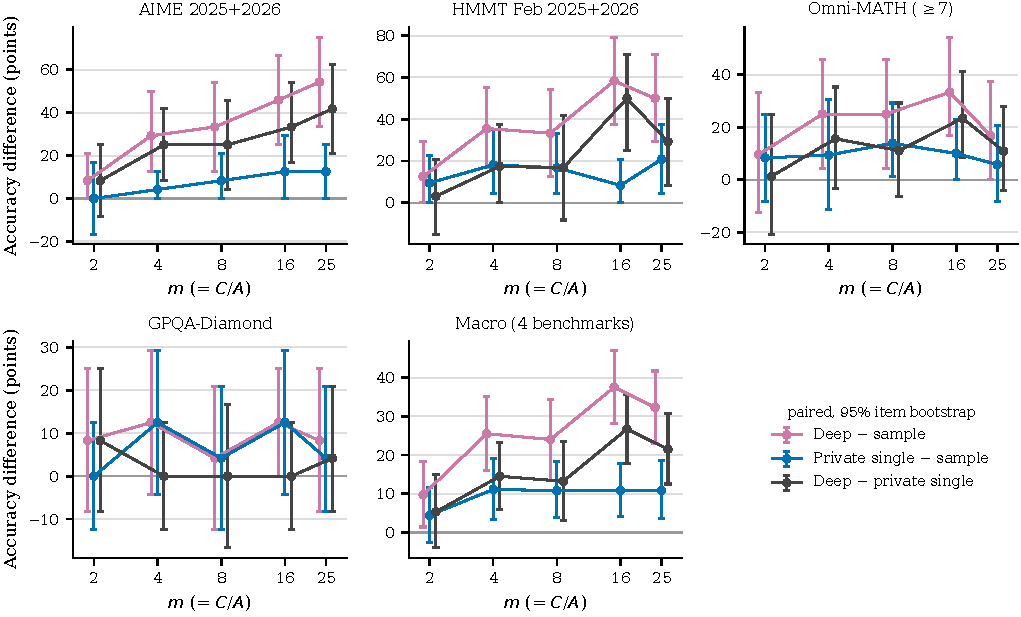
\includegraphics[width=\textwidth]{figures/f3_depth_vs_width.pdf}
\caption{Paired differences at equal realized compute $C = mA$: one deep call minus $m$ samples with a vote,
an $m$-call revision chain minus $m$ samples, and the deep call minus the revision chain. Bars are 95\%
item-clustered bootstrap intervals.}
\label{fig:dvw}
\end{figure}

\begin{table}[htbp]
\centering
\small
\begin{tabular}{rrrrrr}
\toprule
$m$ & macro deep $-$ sample & 95\% CI & deep $-$ private & 95\% CI & private $-$ sample \\ \midrule
2 & +9.7 & [+1.4, +18.2] & +5.3 & [$-$4.0, +14.9] & +4.4 \\
4 & +25.5 & [+15.9, +35.1] & +14.5 & [+5.9, +23.2] & +11.1 \\
8 & +24.0 & [+13.5, +34.4] & +13.2 & [+3.1, +23.6] & +10.8 \\
16 & +37.5 & [+28.1, +46.9] & +26.7 & [+17.7, +35.7] & +10.8 \\
25 & +32.3 & [+22.9, +41.7] & +21.5 & [+12.5, +30.8] & +10.8 \\
\bottomrule
\end{tabular}

\caption{Macro paired differences in accuracy points at equal realized compute $C = mA$.}
\label{tab:dvw}
\end{table}

The comparison also runs across budgets, and there depth wins at a fraction of the cost. A single call at
$4A$ beats twenty-five samples by +18.3 points (95\% CI
+9.8 to +27.1). A call at $8A$ is
+9.0 points above a 25-call revision chain (95\% CI
$-$1.0 to +18.8, so at a third
of the compute it at least matches it). A call at $16A$
beats the best five-agent team at 25 units, \texttt{peer/5/4}, by +21.4
points (95\% CI +13.9 to +29.2).
Per benchmark (Table~\ref{tab:dvwb}) the advantage is largest on HMMT and AIME and vanishes on GPQA-Diamond.

\begin{table}[htbp]
\centering
\small
\begin{tabular}{rlrrrr}
\toprule
$m$ & contrast & AIME & HMMT & Omni & GPQA \\ \midrule
2 & deep $-$ sample & +8.3 & +12.5 & +9.6 & +8.3 \\
2 & deep $-$ private & +8.3 & +3.1 & +1.3 & +8.3 \\
2 & private $-$ sample & +0.0 & +9.4 & +8.3 & +0.0 \\
\addlinespace
4 & deep $-$ sample & +29.2 & +35.5 & +25.0 & +12.5 \\
4 & deep $-$ private & +25.0 & +17.4 & +15.6 & +0.0 \\
4 & private $-$ sample & +4.2 & +18.1 & +9.4 & +12.5 \\
\addlinespace
8 & deep $-$ sample & +33.3 & +33.3 & +25.0 & +4.2 \\
8 & deep $-$ private & +25.0 & +16.7 & +11.1 & +0.0 \\
8 & private $-$ sample & +8.3 & +16.7 & +13.9 & +4.2 \\
\addlinespace
16 & deep $-$ sample & +45.8 & +58.3 & +33.3 & +12.5 \\
16 & deep $-$ private & +33.3 & +50.0 & +23.4 & +0.0 \\
16 & private $-$ sample & +12.5 & +8.3 & +10.0 & +12.5 \\
\addlinespace
25 & deep $-$ sample & +54.2 & +50.0 & +16.7 & +8.3 \\
25 & deep $-$ private & +41.7 & +29.2 & +10.9 & +4.2 \\
25 & private $-$ sample & +12.5 & +20.8 & +5.8 & +4.2 \\
\bottomrule
\end{tabular}

\caption{Per-benchmark paired differences in points at equal realized compute. With 24 items per benchmark
one item is 4.2 points; intervals are in \texttt{numbers.json}.}
\label{tab:dvwb}
\end{table}

\subsection{Scaling trends}
\label{sec:slopes}

Fitting accuracy against $\log_2 C$ from $A$ to $16A$ summarises each family's return on compute
(Figure~\ref{fig:slopes}). On the macro the deep call gains 11.0
points per doubling (95\% CI 8.4 to 13.5); the ceiling of
sampling, pass@$k$, gains 5.7; the revision chain
4.8; and the vote over samples
2.0. The deep call's return per doubling exceeds even the
generation ceiling of sampling: doubling the length of one chain of thought buys more than doubling the
number of independent chains \emph{with perfect selection}. On HMMT the contrast is starkest (deep
14.0, vote 0.2); on
GPQA-Diamond all families scale at similar rates (6.2 for depth,
7.1 for revision).

\begin{figure}[htbp]
\centering
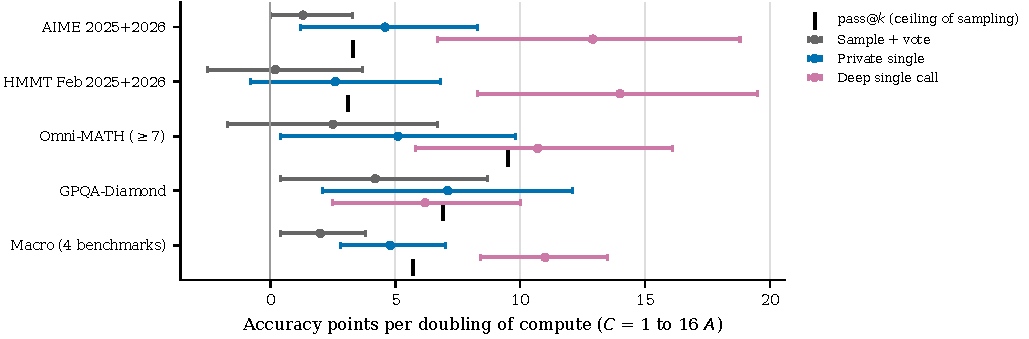
\includegraphics[width=0.85\textwidth]{figures/g8_scaling_slopes.pdf}
\caption{Accuracy points gained per doubling of compute from $C=A$ to $C=16A$ (least-squares slope on
$\log_2 C$; bars are 95\% item-bootstrap intervals). Tick marks: the same slope for pass@$k$, the generation
ceiling of independent sampling.}
\label{fig:slopes}
\end{figure}

\subsection{How revision and communication change answers}
\label{sec:rounds}

The revising trajectories can be followed step by step (Figure~\ref{fig:rounds}). A single agent revising its
own answer converts wrong answers to right ones mostly in its first few steps: the net share of items
corrected at steps 1 to 4 is 0.031, 0.053,
0.022 and 0.022 of items, after which
right-to-wrong changes nearly cancel wrong-to-right ones. Revision without new information saturates quickly,
which is why the chain's accuracy flattens while its archive coverage keeps growing: later steps keep
producing correct answers on some items and discarding them on others.

In teams, net corrections per agent are largest in the first round and decline with rounds for private
teams; for the larger peer teams they stay higher for longer, because an agent that sees a correct peer answer can adopt
it. That is the mechanism behind peer exposure's small positive effect in this study
(Section~\ref{sec:comm}), and it is a selection mechanism: it spreads a correct answer that some agent already
generated, it does not generate a new one.

\begin{figure}[htbp]
\centering
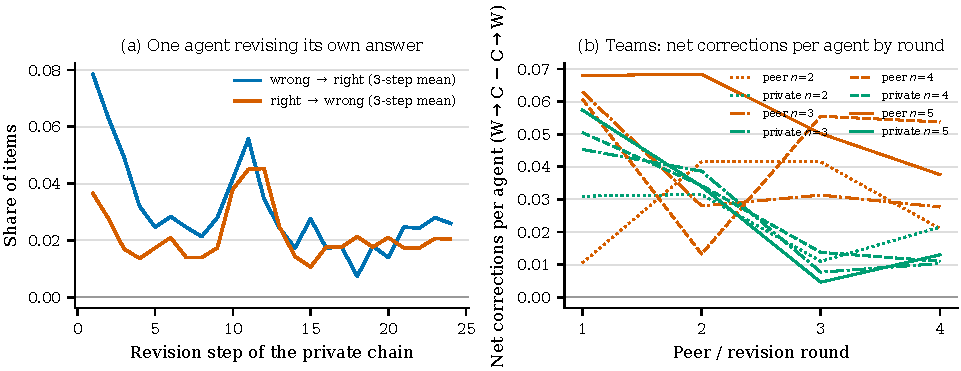
\includegraphics[width=\textwidth]{figures/g7_round_dynamics.pdf}
\caption{(a) Share of items whose answer changes from wrong to right, and from right to wrong, at each step of
the 25-step private chain (3-step moving average). (b) Net corrections (wrong-to-right minus right-to-wrong)
per agent per round, for private and peer teams of each size.}
\label{fig:rounds}
\end{figure}

\subsection{Team shape at equal compute}
\label{sec:shape}

Holding team compute fixed, a team can have more agents or more rounds (Figure~\ref{fig:shape}). The
differences between shapes at the same budget are a few points and mostly within noise, but two regularities
recur: in most budgets up to $12A$, fewer agents with more rounds do at least as well as more agents with
fewer rounds, while at the largest budgets the five-agent peer teams are best. Neither shape comes close to a deep call of the
same budget.

\begin{figure}[htbp]
\centering
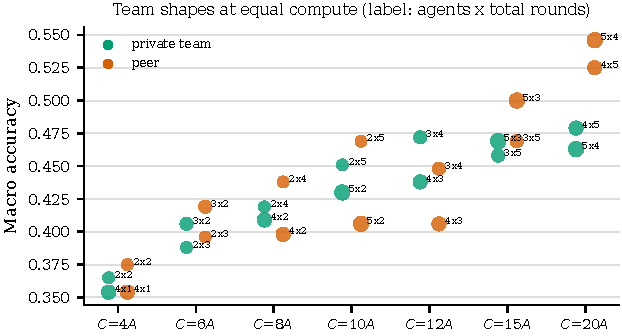
\includegraphics[width=0.72\textwidth]{figures/g9_team_shape.pdf}
\caption{Macro accuracy of teams with the same total compute but different shapes (label: agents $\times$ total
generations per agent, including the initial answer). Marker size grows with the number of agents.}
\label{fig:shape}
\end{figure}

\subsection{The amplification matrix}

Figure~\ref{fig:matrix} compares every allocation with independent sampling at the same budget. On the macro,
25 of 71 comparisons are significantly positive after
Benjamini-Hochberg control and 0 are significantly negative. By family:
4 of 6 deep calls (mean
+21.5 points), 16 of
25 revision chains (mean +9.1),
5 of 20 peer teams (mean
+3.6) and 0 of
20 private teams (mean +2.5).
No allocation does significantly worse than sampling. This is the opposite of v1, where none of 70
per-benchmark comparisons survived correction.

\begin{figure}[htbp]
\centering
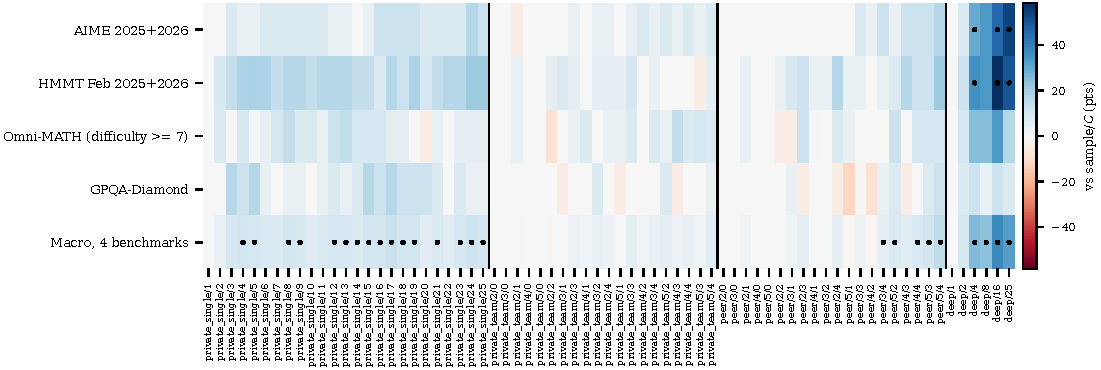
\includegraphics[width=\textwidth]{figures/f5_amplification_matrix.pdf}
\caption{Each allocation minus independent sampling at the same budget, in accuracy points. Dots mark
cells significant after Benjamini-Hochberg control within the row. Columns are grouped by family.}
\label{fig:matrix}
\end{figure}

\subsection{Repetition inside forced calls}
\label{sec:loops}

Forcing a model past the point where it would stop can produce degenerate repetition. We detect a loop as
the first 3,000-character window of the reasoning whose zlib compression ratio falls below 0.1 and count
the reasoning before it as effective depth (Table~\ref{tab:loops}, Figure~\ref{fig:loops}). No 1024-token
call looped. The share of deep calls that loop rises to 0.281 at $16A$ and is
0.208 at $25A$; on average 0.844 of a
$16A$ call's tokens precede any loop.

\begin{table}[htbp]
\centering
\small
\begin{tabular}{rrrrrr}
\toprule
deep/$m$ & reasoning tokens & calls looping & mean effective tokens & effective share & loop onset (median) \\ \midrule
2 & 2,048 & 0.000 & 2,048 & 1.000 & -- \\
4 & 4,096 & 0.052 & 3,950 & 0.965 & 1,243 \\
8 & 8,192 & 0.146 & 7,554 & 0.922 & 3,140 \\
16 & 16,384 & 0.281 & 13,833 & 0.844 & 7,190 \\
25 & 25,600 & 0.208 & 22,319 & 0.872 & 6,701 \\
\bottomrule
\end{tabular}

\caption{Deep calls by forced length. Effective tokens are reasoning before loop onset (all of it for calls
that never loop). Loop onset is the median over looping calls.}
\label{tab:loops}
\end{table}

The loops are not what they appear. A looping call is \emph{more} likely to be correct, not less:
0.963 against 0.725 at $16A$, and
0.950 against 0.697 at $25A$. A call loops when it has
already worked the problem out and has nothing left to do but restate it; the calls that still use the
whole budget productively are the hard ones. The dip from $16A$ to $25A$ on HMMT and Omni-MATH, not
significant on 24 items each, is consistent with this: past the length at which most problems are solved,
extra forced tokens add little and occasionally disturb a finished answer.

\begin{figure}[htbp]
\centering
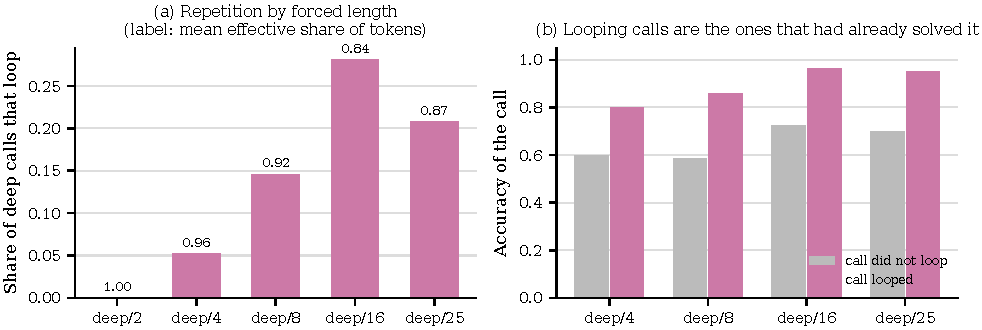
\includegraphics[width=0.85\textwidth]{figures/f8_effective_depth.pdf}
\caption{(a) Share of deep calls whose reasoning degenerates into repetition, labelled with the mean share of
tokens before loop onset. (b) Accuracy of deep calls that looped against those that did not.}
\label{fig:loops}
\end{figure}

\subsection{The cost of letting agents talk}
\label{sec:comm}

In v1, peer exposure destroyed accuracy, increasingly with rounds. Here it helps slightly on average:
across the 16 team shapes peer minus private team averages +1.4 macro points, positive in
11 of 16 cells (Figure~\ref{fig:comm}); at five agents and four rounds it is
+8.5 points (95\% CI +2.7 to +15.1). The frozen
primary contrast at $n=4$, $r=4$ is +4.2 points
on 95 of
96 complete items (sealed bounds
+4.2 to
+5.2); because one item carries an unknown grade
the sealed table withholds a Holm $p$-value, and the known-items paired interval is
$-$2.2 to +11.7 points (Table~\ref{tab:primary}). The gain is
concentrated on HMMT. Either way, every team configuration is far below a single deep call at comparable
or lower cost.

\begin{figure}[htbp]
\centering
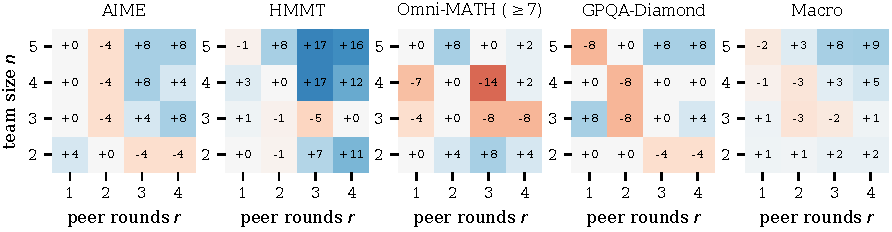
\includegraphics[width=\textwidth]{figures/f7_communication.pdf}
\caption{Peer minus private team, in accuracy points, by team size and number of peer rounds. Both arms
spend identical compute; only exposure to peers differs.}
\label{fig:comm}
\end{figure}

\begin{table}[htbp]
\centering
\small
\begin{tabular}{lrrrr}
\toprule
Contrast (sealed, frozen before collection) & estimate (pts) & bounds (pts) & complete & status \\ \midrule
(i) peer/4/4 $-$ private\_team/4/4 & +4.2 & [+4.2, +5.2] & 95/96 & partial \\
(ii) CP gain $-$ private-team gain, $h$=3 & +1.1 & [+0.0, +2.1] & 94/96 & partial \\
\bottomrule
\end{tabular}

\caption{The two contrasts frozen before collection, as sealed. ``partial'' means some items carry an
unknown grade: the estimate is over complete items and the bounds fix every unknown term at its extremes.}
\label{tab:primary}
\end{table}

\subsection{What this costs in dollars}

Realized compute and dollars are close to proportional in this design, but not exactly: a deep call pays
for its long reasoning once, while a revision chain or a team re-reads prompts and candidate packets on
every call. The accuracy-per-dollar frontier (Figure~\ref{fig:dollars}) consists entirely of deep calls:
\texttt{deep/16} delivers 0.792 at 0.044 dollars per item, while
\texttt{sample/25} delivers 0.427 at 0.093 and \texttt{peer/5/4}
delivers 0.577 at 0.108.

\begin{figure}[htbp]
\centering
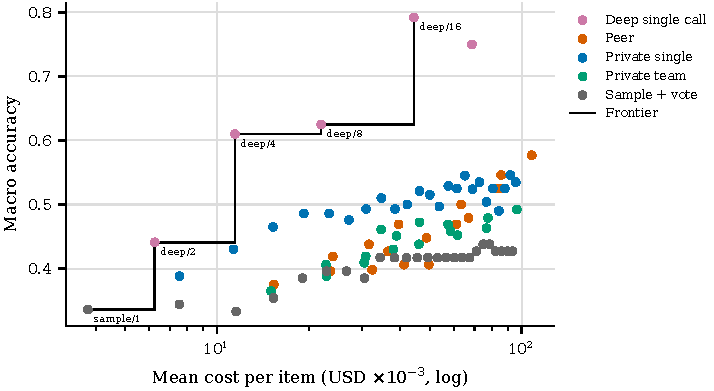
\includegraphics[width=0.7\textwidth]{figures/f9_dollars.pdf}
\caption{Macro accuracy against mean generation cost per item (all calls of the configuration, both THINK
and ANSWER). The step line is the frontier of configurations not dominated on both axes.}
\label{fig:dollars}
\end{figure}

\subsection{Robustness}

The two providers served disjoint items, so provider is a covariate, not a paired contrast. The depth
advantage appears on both (Figure~\ref{fig:rob}): deep/16 minus sample/16 is
+39.7 points on Mancer's 58 items
and +34.2 on Parasail's 38,
although the two item sets differ in difficulty (pass@1 0.281 and
0.421). Unknown grades affect 46 configuration outcomes
on two items; each item is about one macro point, so they cannot move any macro comparison above by more than about two points.

\begin{figure}[htbp]
\centering
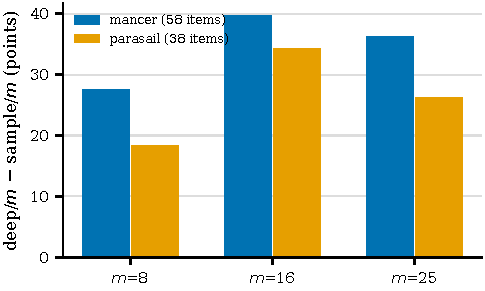
\includegraphics[width=0.5\textwidth]{figures/f10_robustness.pdf}
\caption{deep/$m$ minus sample/$m$ within each provider's items.}
\label{fig:rob}
\end{figure}

\section{Interpretation}

\paragraph{The generation-selection gap depends on what you measure it against.} v1 measured the gap against
pass@$k$ of the samples it drew and found that selection was the bottleneck. That is true of independent
sampling in every regime: vote@$k$ sits well below pass@$k$ here too, by 17.6
macro points at $k=25$. But pass@$k$ at a fixed per-call budget is the ceiling of one allocation, not of the
compute. Once the per-call budget can be spent on depth, the relevant ceiling moves: one 16,384-token call
delivers more than a perfect selector over sixteen 1024-token calls could. The gap between short samples and
depth is a generation gap that pass@$k$ at $A$ conceals.

\paragraph{Structured allocation can close the gap only by changing what is generated.} The multi-call
structures in the design (revision chains, private and peer teams, communicate-then-private, pooled synthesis)
raise generation modestly above the sampling ceiling but lose most of it at selection, and no verifier over
their candidates reaches depth. The single deep call closes the gap by construction, because it generates and
selects in one step, and it overshoots the sampling ceiling because it reaches answers short samples never
produce. A structured approach that works therefore has two stages: concentrate compute in depth until the
per-call budget is no longer binding, and only then spend on width and selection.

\paragraph{The regime is set by the ratio of budget to required reasoning.} Where short calls already reach the
answer (GPQA-Diamond here, the easy benchmarks of v1), depth adds little, the gap is a genuine selection gap,
and verification is the lever. Where they do not (AIME, HMMT), depth dominates. The item-level analysis shows
that this is a property of items, not only of benchmarks, and that the agreement among a handful of short
samples is a cheap signal of which regime an item is in.

\paragraph{Mechanisms.} Revision helps early and then churns; peer exposure spreads correct answers it already
has; deep calls of different lengths are highly correlated; and long forced calls fall into repetition mainly
once they are done. All of these point the same way: returns come from lengthening a single productive line
of reasoning, and from width only once that line is long enough.

\paragraph{Limits.} This is one 27B model on 96 items, 24 per benchmark. The deep calls are single samples, so
the portfolio analysis cannot measure the diversity of repeated calls at one depth. Forcing is a decode-time
intervention: a forced call is not the call the model would choose, and its value depends on the model's
ability to use a long budget, which is a property of its training.

\section{What to do with this}

\begin{enumerate}
\item \textbf{Measure the per-call budget against the reasoning the task needs before allocating.} The forcing
mechanism and a small unforced calibration give the natural reasoning length cheaply. If it exceeds the
per-call budget, raise the budget before adding calls: on this mix a call at $4A$ beat twenty-five calls at $A$
by 18.3 points.
\item \textbf{Route by agreement.} Draw a few short samples; if they agree, deliver the plurality (it is almost
always right when it holds a large share); if they scatter, spend the remaining budget on one deep call. (This rule is suggested by the data here and should be tested
prospectively; see Section~\ref{sec:follow}.)
\item \textbf{Do not expect selection to rescue short samples on hard problems.} Even perfect verification over
short samples stays below depth in this regime; invest in verification where short samples already generate
the answer (the GPQA regime), which is where v1's prescription still applies.
\item \textbf{Use revision as the second lever, and stop early.} Its gains come in the first few steps; a long
revision chain mostly churns.
\end{enumerate}

\section{A follow-up experiment: width at depth}
\label{sec:follow}

The open question is the one this design could not answer: once depth is sufficient, does width pay again? The
experiment is the full width-by-depth grid of \emph{independent} calls: $k$ calls of $mA$ each with $km = C$,
read out by vote, by the agreement-routing rule above, and by a verifier, for $C = 16A$ and $32A$. It reuses
this run's items, prompts, forcing, grading and analysis, and the one deep call per depth already collected.
For $C=16A$ it needs 7 new calls at $2A$, 3 at $4A$ and 1 at $8A$ per item; for $C=32A$ 15 at $2A$, 7 at $4A$,
3 at $8A$ and 1 at $16A$: 37 calls and 135,168 forced
reasoning tokens per item. At this run's measured cost per call that is about \$0.38 per
item, or about \$36.84 for the 96-item panel. It would locate the optimum $(k, m)$ at
each budget, measure the diversity of repeated deep calls that the portfolio analysis could not, and test
agreement routing prospectively.

\appendix
\section{Run facts}

Total generation cost \$70.00 (accepted generations), of which the main run
\$65.24; OpenRouter key usage over the study window \$70.33. The ledger
charged \$72.26, above key usage because \$2.19 of ambiguous
attempts were conservatively charged at their full reservation; its invariant checks recorded
0 violations. Canary \$0.70, calibration
\$1.76, pilot \$2.30. The main run dispatched
13,344 generation nodes, each two HTTP calls, over two concurrent provider shards in
about 1.6 hours; median visible answer length was 321 tokens. All pre-registered gates
passed, with two notes. The canary's check of the ledger against provider usage first failed because both
shards bill one key concurrently, so each shard's usage window contained the other's spend; it was
re-evaluated over the union of the windows against the sum of both ledgers, and passed. And there were two
owner-accepted exceptions on the Mancer pilot (AIME invalid finals at 94.4\% against 95\%,
and a forecast above that shard's proportional budget slice, resolved by re-splitting the \$95 cap).
Sealed tables, the merge manifest and every figure and number in this report are regenerated by
\texttt{build.sh} from the run directory.

\section{Every configuration at every depth budget}
\label{app:full}

Macro delivered accuracy, current-pool and archive coverage, archive selection gap (coverage minus delivered)
and the difference from pass@$k$ at $A$, for every configuration at the five budgets that carry a deep call.
$|$pool$|$ is the number of candidates in the archive pool. Differences are in accuracy points.

{\small
\begin{longtable}{rlrrrrrr}
\toprule
$C/A$ & configuration & $|$pool$|$ & delivered & cov.\ (current) & cov.\ (all) & gap (all) & $-$ pass@$k$ \\
\midrule
\endhead
\multicolumn{8}{l}{\emph{$C=2A$: pass@2 = 0.422, prefix coverage = 0.440}} \\
2 & \texttt{sample/2} & 2 & 0.344 & 0.440 & 0.440 & +9.6 & $-$7.9 \\
2 & \texttt{private\_single/2} & 2 & 0.388 & 0.388 & 0.430 & +4.2 & $-$3.4 \\
2 & \texttt{private\_team/2/0} & 2 & 0.344 & 0.440 & 0.440 & +9.6 & $-$7.9 \\
2 & \texttt{peer/2/0} & 2 & 0.344 & 0.440 & 0.440 & +9.6 & $-$7.9 \\
2 & \texttt{deep/2} & 1 & 0.441 & 0.441 & 0.441 & +0.0 & +1.8 \\
\addlinespace
\multicolumn{8}{l}{\emph{$C=4A$: pass@4 = 0.484, prefix coverage = 0.465}} \\
4 & \texttt{sample/4} & 4 & 0.354 & 0.465 & 0.465 & +11.1 & $-$13.0 \\
4 & \texttt{private\_single/4} & 4 & 0.465 & 0.465 & 0.540 & +7.5 & $-$1.9 \\
4 & \texttt{private\_team/2/1} & 4 & 0.365 & 0.492 & 0.524 & +15.9 & $-$11.9 \\
4 & \texttt{private\_team/4/0} & 4 & 0.354 & 0.465 & 0.465 & +11.1 & $-$13.0 \\
4 & \texttt{peer/2/1} & 4 & 0.375 & 0.427 & 0.471 & +9.6 & $-$10.9 \\
4 & \texttt{peer/4/0} & 4 & 0.354 & 0.465 & 0.465 & +11.1 & $-$13.0 \\
4 & \texttt{deep/4} & 1 & 0.610 & 0.610 & 0.610 & +0.0 & +12.6 \\
\addlinespace
\multicolumn{8}{l}{\emph{$C=8A$: pass@8 = 0.536, prefix coverage = 0.540}} \\
8 & \texttt{sample/8} & 8 & 0.385 & 0.540 & 0.540 & +15.4 & $-$15.0 \\
8 & \texttt{private\_single/8} & 8 & 0.493 & 0.493 & 0.561 & +6.8 & $-$4.2 \\
8 & \texttt{private\_team/2/3} & 8 & 0.419 & 0.507 & 0.603 & +18.4 & $-$11.6 \\
8 & \texttt{private\_team/4/1} & 8 & 0.409 & 0.543 & 0.566 & +15.7 & $-$12.7 \\
8 & \texttt{peer/2/3} & 8 & 0.438 & 0.469 & 0.535 & +9.7 & $-$9.8 \\
8 & \texttt{peer/4/1} & 8 & 0.398 & 0.498 & 0.529 & +13.1 & $-$13.8 \\
8 & \texttt{deep/8} & 1 & 0.625 & 0.625 & 0.625 & +0.0 & +8.9 \\
8 & \texttt{cp/0} & 8 & 0.398 & 0.498 & 0.529 & +13.1 & $-$13.8 \\
8 & \texttt{pooled/4} & 5 & 0.412 & 0.412 & 0.509 & +9.6 & $-$12.3 \\
\addlinespace
\multicolumn{8}{l}{\emph{$C=16A$: pass@16 = 0.580, prefix coverage = 0.571}} \\
16 & \texttt{sample/16} & 16 & 0.417 & 0.571 & 0.571 & +15.4 & $-$16.3 \\
16 & \texttt{private\_single/16} & 16 & 0.525 & 0.525 & 0.657 & +13.2 & $-$5.5 \\
16 & \texttt{private\_team/4/3} & 16 & 0.452 & 0.582 & 0.640 & +18.8 & $-$12.7 \\
16 & \texttt{peer/4/3} & 16 & 0.479 & 0.557 & 0.615 & +13.6 & $-$10.0 \\
16 & \texttt{deep/16} & 1 & 0.792 & 0.792 & 0.792 & +0.0 & +21.2 \\
16 & \texttt{cp/2} & 16 & 0.427 & 0.555 & 0.614 & +18.7 & $-$15.3 \\
\addlinespace
\multicolumn{8}{l}{\emph{$C=25A$: pass@25 = 0.603, prefix coverage = 0.603}} \\
25 & \texttt{sample/25} & 25 & 0.427 & 0.603 & 0.603 & +17.6 & $-$17.6 \\
25 & \texttt{private\_single/25} & 25 & 0.535 & 0.535 & 0.689 & +15.4 & $-$6.8 \\
25 & \texttt{private\_team/5/4} & 25 & 0.492 & 0.588 & 0.662 & +17.0 & $-$11.1 \\
25 & \texttt{peer/5/4} & 25 & 0.577 & 0.599 & 0.647 & +6.9 & $-$2.6 \\
25 & \texttt{deep/25} & 1 & 0.750 & 0.750 & 0.750 & +0.0 & +14.7 \\
\addlinespace
\bottomrule
\end{longtable}

}

\end{document}
